
\section{Question 3}
Tìm vị trí các parking slot còn trống trong hình
\begin{figure}[H]
    \centering
    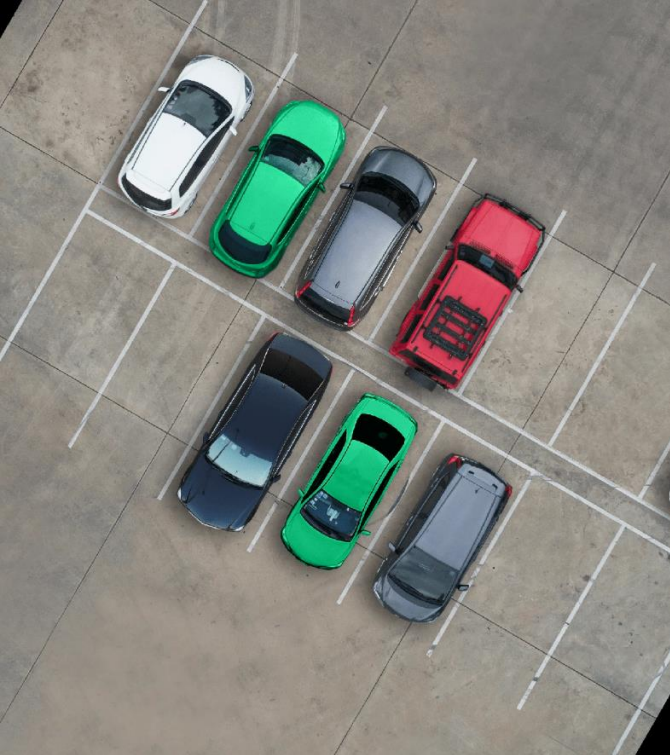
\includegraphics[width=0.7\textwidth]{pictures/chapter3/s3_p01.png}
    \caption{Ảnh đề bài}
    \label{fig:label}
\end{figure}

\subsection{Quy trình thực hiện}

\subsubsection*{Bước 1: Tiền xử lý và ước lượng góc nghiêng}
Do ảnh bãi đỗ xe thường được chụp từ góc nghiêng, việc đầu tiên cần làm là xác định góc nghiêng của bãi xe.

\textbf{Các bước thực hiện:}
\begin{itemize}
    \item Resize ảnh về kích thước phù hợp (MAX\_SIDE\_PX = 900) để tăng tốc độ xử lý
    \item Áp dụng Gaussian Blur và Canny Edge Detection để phát hiện các cạnh trong ảnh
    \item Sử dụng Hough Transform để phát hiện các đường thẳng chính trong ảnh
    \item Tính góc trung vị của các đường thẳng chéo (không gần 0° hoặc 90°) để xác định góc nghiêng chính
\end{itemize}

\subsubsection*{Bước 2: Xoay ảnh}
Sau khi tính được góc nghiêng chính, tiến hành xoay ảnh về vị trí thẳng đứng để thuận tiện cho việc phát hiện vạch kẻ.

\textbf{Công thức xoay ảnh:}
\begin{equation}
    M = \begin{bmatrix} 
    \cos\theta & -\sin\theta & t_x \\ 
    \sin\theta & \cos\theta & t_y 
    \end{bmatrix}
\end{equation}

Với $\theta = \text{main\_angle} - 90°$, và tâm xoay là tâm ảnh.
\begin{lstlisting}[language=Python]
def rotate_image(img, angle_deg):
    h, w = img.shape[:2]
    center = (w // 2, h // 2)
    M = cv2.getRotationMatrix2D(center, angle_deg, 1.0)
    rotated = cv2.warpAffine(img, M, (w, h), flags=cv2.INTER_LINEAR)
    return rotated, M
\end{lstlisting}
\begin{figure}[H]
    \centering
    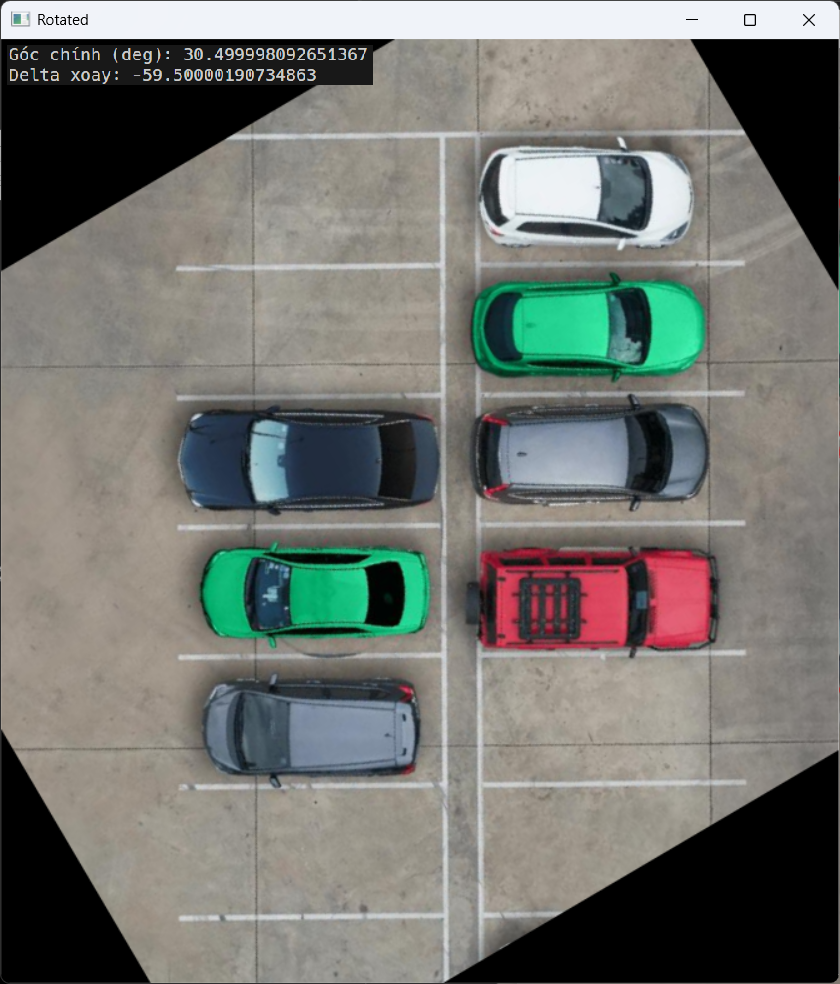
\includegraphics[width=0.7\textwidth]{pictures/chapter3/s3_p02.png}
    \caption{Kết quả ảnh sau khi xoay}
    \label{fig:label}
\end{figure}
\cleardoublepage
\subsubsection*{Bước 3: Phát hiện lưới các ô đỗ xe từ vạch trắng (detect\_grid\_slots\_from\_img)}
Đây là bước quan trọng nhất, bao gồm nhiều công đoạn nhỏ để phát hiện và tạo lưới các ô đỗ xe.

\textbf{3.1. Phát hiện vùng trắng bằng không gian màu HLS:}
\begin{itemize}
    \item Chuyển ảnh từ BGR sang HLS (Hue-Lightness-Saturation)
    \item Tạo mask cho vùng có độ sáng cao: $L \geq 165$
    \item Tạo mask cho vùng có độ bão hòa thấp: $S \leq 160$
    \item Kết hợp hai mask để lọc vùng trắng/xám sáng
\end{itemize}

\textbf{3.2. Bổ sung phát hiện từ ảnh grayscale:}
\begin{itemize}
    \item Áp dụng Canny Edge trên ảnh grayscale
    \item Tạo mask cho pixel sáng: $\text{gray} \geq 170$
    \item Kết hợp với edge để phát hiện các vạch mờ
\end{itemize}

\textbf{3.3. Xử lý hình học:}
\begin{itemize}
    \item Morphological Close: nối các vạch gần nhau
    \item Morphological Open: loại bỏ nhiễu nhỏ
\end{itemize}

\textbf{3.4. Phát hiện đường thẳng bằng Hough Transform:}
Áp dụng HoughLinesP (Probabilistic Hough Line Transform) trên ảnh edge để phát hiện các đoạn thẳng.

\textbf{Tham số:}
\begin{itemize}
    \item Threshold: 30 (số điểm tối thiểu trên một đường thẳng)
    \item minLineLength: 50 pixels (độ dài tối thiểu)
    \item maxLineGap: 30 pixels (khoảng cách tối đa giữa các đoạn để nối thành một đường)
\end{itemize}

\textbf{Phân loại đường thẳng:}
\begin{itemize}
    \item Đường ngang: $|\theta| < 30°$
    \item Đường dọc: $60° < |\theta| < 120°$
\end{itemize}

\textbf{3.5. Tinh chỉnh vị trí vạch dọc:}
Để cải thiện độ chính xác, vị trí các vạch dọc được tinh chỉnh bằng cách:
\begin{enumerate}
    \item Lấy vùng dưới cùng của ảnh (từ 60\% chiều cao trở xuống)
    \item Với mỗi vạch dọc được phát hiện, tìm kiếm trong vùng $\pm 70$ pixels
    \item Tính tổng pixel trắng theo từng cột trong vùng tìm kiếm
    \item Chọn cột có tổng pixel trắng cao nhất làm vị trí chính xác của vạch
\end{enumerate}

\textbf{Xử lý trường hợp đặc biệt:} Nếu chỉ phát hiện được 2 vạch dọc, hệ thống tự động sinh thêm 1 vạch bên trái với khoảng cách bằng khoảng cách giữa 2 vạch hiện có.

\textbf{3.6. Tạo lưới các ô đỗ xe:}
Từ tập hợp các vạch ngang ($y_i$) và vạch dọc ($x_j$), tạo các ô chữ nhật:
\begin{equation}
    \text{Slot}_{ij} = (x_i, y_j, x_{i+1}, y_{j+1})
\end{equation}

Lọc bỏ các ô có kích thước quá nhỏ:
\begin{itemize}
    \item $\text{width} < 20$ pixels
    \item $\text{height} < 20$ pixels
\end{itemize}
\begin{figure}[H]
    \centering
    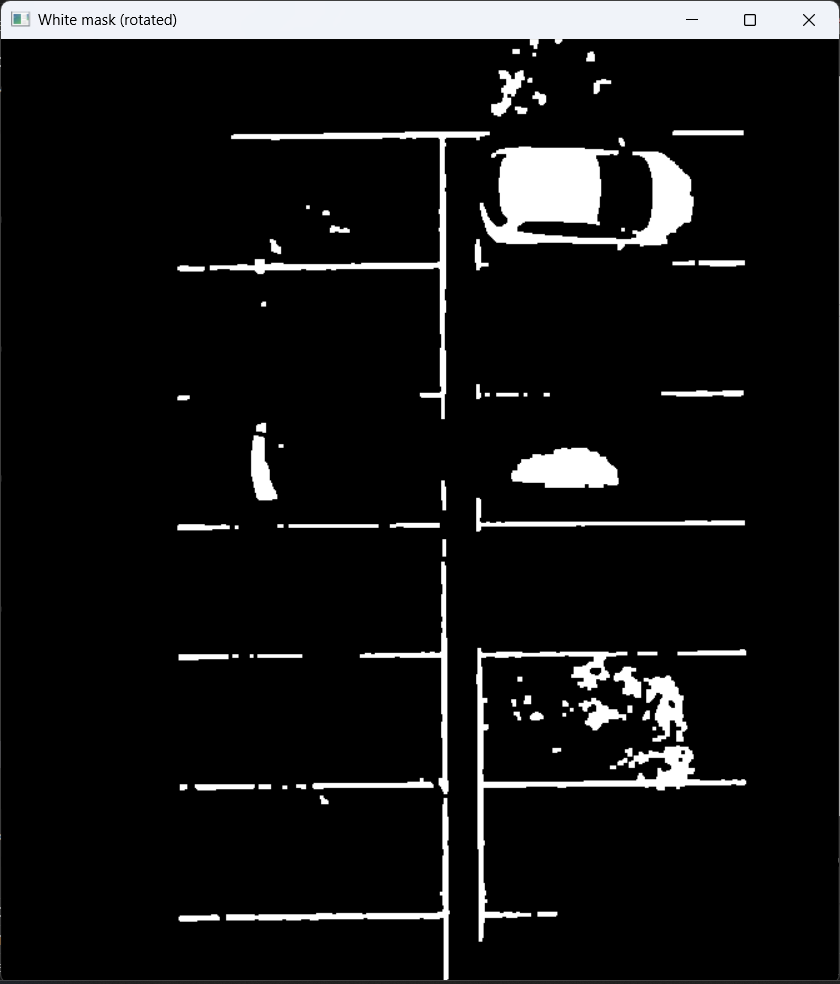
\includegraphics[width=0.7\textwidth]{pictures/chapter3/s3_p03.png}
    \caption{Kết quả ảnh ở bước phát hiện vạch ô đỗ xe}
    \label{fig:label}
\end{figure}
\subsubsection*{Bước 4: Phân loại ô trống và ô có xe (classify\_slots)}
Sử dụng kênh Saturation (S) trong không gian màu HSV để phân biệt ô trống và ô có xe.

\textbf{Nguyên lý:}
\begin{itemize}
    \item Xe thường có màu sắc đa dạng $\Rightarrow$ độ bão hòa cao
    \item Ô trống (mặt đường xám) $\Rightarrow$ độ bão hòa thấp
\end{itemize}

\textbf{Thuật toán:}
\begin{enumerate}
    \item Chuyển ROI của mỗi slot sang HSV
    \item Tạo mask cho pixel có $S > 50$
    \item Áp dụng morphological operations để làm mịn mask
    \item Tính tỷ lệ pixel có màu: $\text{ratio} = \frac{\sum \text{mask}}{w \times h}$
    \item Phân loại:
    \begin{equation}
        \text{Trạng thái} = \begin{cases} 
        \text{Có xe} & \text{nếu ratio} > 0.12 \\
        \text{Trống} & \text{nếu ratio} \leq 0.12
        \end{cases}
    \end{equation}
\end{enumerate}
\begin{lstlisting}[language=Python]
def classify_slots(rot_img, slots,
                   s_thresh=50,
                   area_ratio_thresh=0.12):
    occupied = []
    empty    = []

    for (x1, y1, x2, y2) in slots:
        slot = rot_img[y1:y2, x1:x2]
        if slot.size == 0:
            continue

        hsv = cv2.cvtColor(slot, cv2.COLOR_BGR2HSV)
        _, S, _ = cv2.split(hsv)

        mask = (S > s_thresh).astype(np.uint8)

        kernel = np.ones((3, 3), np.uint8)
        mask = cv2.morphologyEx(mask, cv2.MORPH_OPEN, kernel, 1)
        mask = cv2.morphologyEx(mask, cv2.MORPH_CLOSE, kernel, 1)

        ratio = mask.mean()  # 0..1

        if ratio > area_ratio_thresh:
            occupied.append((x1, y1, x2, y2, ratio))
        else:
            empty.append((x1, y1, x2, y2, ratio))

    return occupied, empty
\end{lstlisting}
\cleardoublepage
\subsubsection*{Bước 5: Vẽ kết quả trên ảnh đã xoay (draw\_result)}
Vẽ các ô đỗ xe trên ảnh đã xoay:
\begin{itemize}
    \item Vẽ hình chữ nhật màu đỏ cho ô có xe
    \item Vẽ hình chữ nhật màu xanh lá cho ô trống
\end{itemize}
\begin{lstlisting}{language=Python}
    def draw_result(rot_img, occupied, empty):
    out = rot_img.copy()

    for (x1, y1, x2, y2, _) in occupied:
        cv2.rectangle(out, (x1, y1), (x2, y2), (0, 0, 255), 2)  

    for (x1, y1, x2, y2, _) in empty:
        cv2.rectangle(out, (x1, y1), (x2, y2), (0, 255, 0), 2)  

    return out
\end{lstlisting}
\begin{figure}[H]
    \centering
    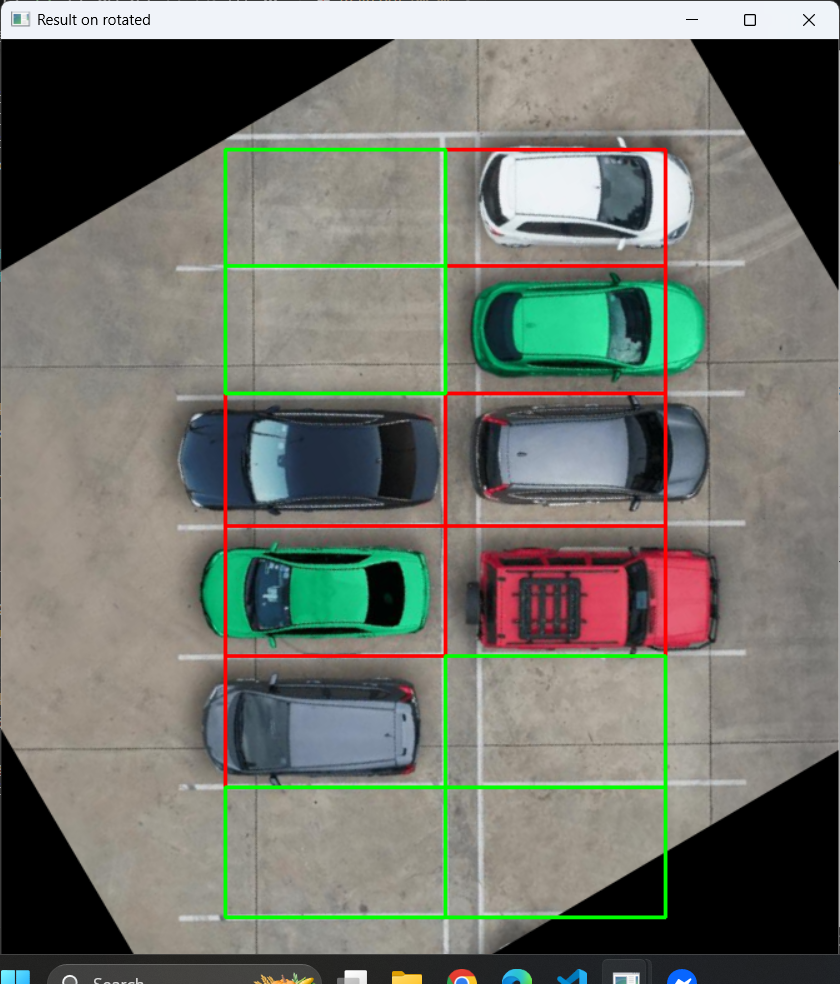
\includegraphics[width=0.7\textwidth]{pictures/chapter3/s3_p04.png}
    \caption{Kết quả các ô đỗ xe trên ảnh đã xoay}
    \label{fig:label}
\end{figure}
\cleardoublepage
\subsubsection*{Bước 6: Vẽ kết quả về ảnh gốc (draw\_on\_original)}
Hiển thị kết quả trên ảnh gốc (chưa xoay):
\begin{itemize}
    \item Sử dụng ma trận nghịch đảo $M^{-1}$ để biến đổi 4 góc của mỗi ô về hệ tọa độ gốc
    \item Vẽ đa giác (polylines) màu đỏ/xanh tương ứng
\end{itemize}
\begin{lstlisting}{language=Python}
    def transform_points_quad(x1, y1, x2, y2, M_inv):
    pts_rot = np.array([[
        [x1, y1],
        [x2, y1],
        [x2, y2],
        [x1, y2]
    ]], dtype=np.float32)  # (1,4,2)

    pts_orig = cv2.transform(pts_rot, M_inv)
    pts_orig = np.round(pts_orig).astype(np.int32)
    return pts_orig[0]  # (4,2)


def draw_on_original(orig_img, occupied, empty, M_inv):
    out = orig_img.copy()

    for (x1, y1, x2, y2, _) in empty:
        quad = transform_points_quad(x1, y1, x2, y2, M_inv)
        cv2.polylines(out, [quad.reshape((-1, 1, 2))],
                      isClosed=True, color=(0, 255, 0), thickness=2)

    for (x1, y1, x2, y2, _) in occupied:
        quad = transform_points_quad(x1, y1, x2, y2, M_inv)
        cv2.polylines(out, [quad.reshape((-1, 1, 2))],
                      isClosed=True, color=(0, 0, 255), thickness=2)

    return out
\end{lstlisting}
\begin{figure}[H]
    \centering
    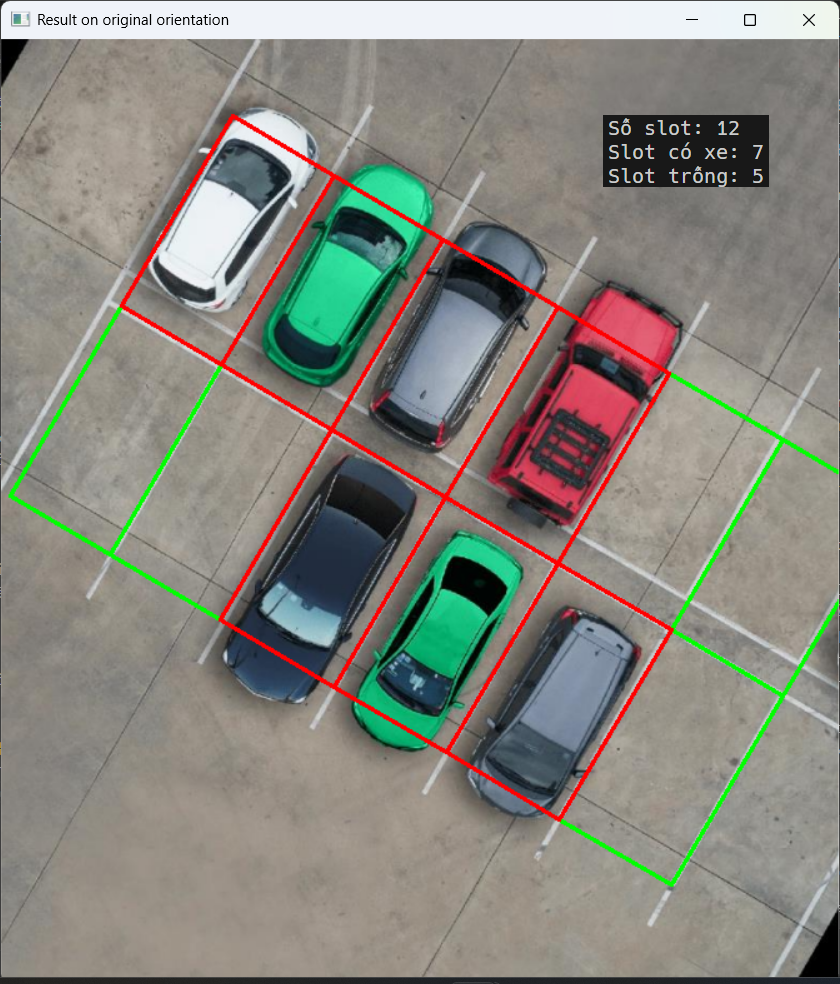
\includegraphics[width=1\textwidth]{pictures/chapter3/s3_p05.png}
    \caption{Kết quả các ô đỗ xe trên ảnh gốc}
    \label{fig:label}
\end{figure}
\cleardoublepage
